% Options for packages loaded elsewhere
% Options for packages loaded elsewhere
\PassOptionsToPackage{unicode}{hyperref}
\PassOptionsToPackage{hyphens}{url}
\PassOptionsToPackage{dvipsnames,svgnames,x11names}{xcolor}
%
\documentclass[
  letterpaper,
  DIV=11,
  numbers=noendperiod]{scrartcl}
\usepackage{xcolor}
\usepackage[margin=1in]{geometry}
\usepackage{amsmath,amssymb}
\setcounter{secnumdepth}{-\maxdimen} % remove section numbering
\usepackage{iftex}
\ifPDFTeX
  \usepackage[T1]{fontenc}
  \usepackage[utf8]{inputenc}
  \usepackage{textcomp} % provide euro and other symbols
\else % if luatex or xetex
  \usepackage{unicode-math} % this also loads fontspec
  \defaultfontfeatures{Scale=MatchLowercase}
  \defaultfontfeatures[\rmfamily]{Ligatures=TeX,Scale=1}
\fi
\usepackage{lmodern}
\ifPDFTeX\else
  % xetex/luatex font selection
\fi
% Use upquote if available, for straight quotes in verbatim environments
\IfFileExists{upquote.sty}{\usepackage{upquote}}{}
\IfFileExists{microtype.sty}{% use microtype if available
  \usepackage[]{microtype}
  \UseMicrotypeSet[protrusion]{basicmath} % disable protrusion for tt fonts
}{}
\makeatletter
\@ifundefined{KOMAClassName}{% if non-KOMA class
  \IfFileExists{parskip.sty}{%
    \usepackage{parskip}
  }{% else
    \setlength{\parindent}{0pt}
    \setlength{\parskip}{6pt plus 2pt minus 1pt}}
}{% if KOMA class
  \KOMAoptions{parskip=half}}
\makeatother
% Make \paragraph and \subparagraph free-standing
\makeatletter
\ifx\paragraph\undefined\else
  \let\oldparagraph\paragraph
  \renewcommand{\paragraph}{
    \@ifstar
      \xxxParagraphStar
      \xxxParagraphNoStar
  }
  \newcommand{\xxxParagraphStar}[1]{\oldparagraph*{#1}\mbox{}}
  \newcommand{\xxxParagraphNoStar}[1]{\oldparagraph{#1}\mbox{}}
\fi
\ifx\subparagraph\undefined\else
  \let\oldsubparagraph\subparagraph
  \renewcommand{\subparagraph}{
    \@ifstar
      \xxxSubParagraphStar
      \xxxSubParagraphNoStar
  }
  \newcommand{\xxxSubParagraphStar}[1]{\oldsubparagraph*{#1}\mbox{}}
  \newcommand{\xxxSubParagraphNoStar}[1]{\oldsubparagraph{#1}\mbox{}}
\fi
\makeatother


\usepackage{longtable,booktabs,array}
\newcounter{none} % for unnumbered tables
\usepackage{calc} % for calculating minipage widths
% Correct order of tables after \paragraph or \subparagraph
\usepackage{etoolbox}
\makeatletter
\patchcmd\longtable{\par}{\if@noskipsec\mbox{}\fi\par}{}{}
\makeatother
% Allow footnotes in longtable head/foot
\IfFileExists{footnotehyper.sty}{\usepackage{footnotehyper}}{\usepackage{footnote}}
\makesavenoteenv{longtable}
\usepackage{graphicx}
\makeatletter
\newsavebox\pandoc@box
\newcommand*\pandocbounded[1]{% scales image to fit in text height/width
  \sbox\pandoc@box{#1}%
  \Gscale@div\@tempa{\textheight}{\dimexpr\ht\pandoc@box+\dp\pandoc@box\relax}%
  \Gscale@div\@tempb{\linewidth}{\wd\pandoc@box}%
  \ifdim\@tempb\p@<\@tempa\p@\let\@tempa\@tempb\fi% select the smaller of both
  \ifdim\@tempa\p@<\p@\scalebox{\@tempa}{\usebox\pandoc@box}%
  \else\usebox{\pandoc@box}%
  \fi%
}
% Set default figure placement to htbp
\def\fps@figure{htbp}
\makeatother


% definitions for citeproc citations
\NewDocumentCommand\citeproctext{}{}
\NewDocumentCommand\citeproc{mm}{%
  \begingroup\def\citeproctext{#2}\cite{#1}\endgroup}
\makeatletter
 % allow citations to break across lines
 \let\@cite@ofmt\@firstofone
 % avoid brackets around text for \cite:
 \def\@biblabel#1{}
 \def\@cite#1#2{{#1\if@tempswa , #2\fi}}
\makeatother
\newlength{\cslhangindent}
\setlength{\cslhangindent}{1.5em}
\newlength{\csllabelwidth}
\setlength{\csllabelwidth}{3em}
\newenvironment{CSLReferences}[2] % #1 hanging-indent, #2 entry-spacing
 {\begin{list}{}{%
  \setlength{\itemindent}{0pt}
  \setlength{\leftmargin}{0pt}
  \setlength{\parsep}{0pt}
  % turn on hanging indent if param 1 is 1
  \ifodd #1
   \setlength{\leftmargin}{\cslhangindent}
   \setlength{\itemindent}{-1\cslhangindent}
  \fi
  % set entry spacing
  \setlength{\itemsep}{#2\baselineskip}}}
 {\end{list}}
\usepackage{calc}
\newcommand{\CSLBlock}[1]{\hfill\break\parbox[t]{\linewidth}{\strut\ignorespaces#1\strut}}
\newcommand{\CSLLeftMargin}[1]{\parbox[t]{\csllabelwidth}{\strut#1\strut}}
\newcommand{\CSLRightInline}[1]{\parbox[t]{\linewidth - \csllabelwidth}{\strut#1\strut}}
\newcommand{\CSLIndent}[1]{\hspace{\cslhangindent}#1}



\setlength{\emergencystretch}{3em} % prevent overfull lines

\providecommand{\tightlist}{%
  \setlength{\itemsep}{0pt}\setlength{\parskip}{0pt}}



 


\KOMAoption{captions}{tableheading}
\makeatletter
\@ifpackageloaded{tcolorbox}{}{\usepackage[skins,breakable]{tcolorbox}}
\@ifpackageloaded{fontawesome5}{}{\usepackage{fontawesome5}}
\definecolor{quarto-callout-color}{HTML}{909090}
\definecolor{quarto-callout-note-color}{HTML}{0758E5}
\definecolor{quarto-callout-important-color}{HTML}{CC1914}
\definecolor{quarto-callout-warning-color}{HTML}{EB9113}
\definecolor{quarto-callout-tip-color}{HTML}{00A047}
\definecolor{quarto-callout-caution-color}{HTML}{FC5300}
\definecolor{quarto-callout-color-frame}{HTML}{acacac}
\definecolor{quarto-callout-note-color-frame}{HTML}{4582ec}
\definecolor{quarto-callout-important-color-frame}{HTML}{d9534f}
\definecolor{quarto-callout-warning-color-frame}{HTML}{f0ad4e}
\definecolor{quarto-callout-tip-color-frame}{HTML}{02b875}
\definecolor{quarto-callout-caution-color-frame}{HTML}{fd7e14}
\makeatother
\makeatletter
\@ifpackageloaded{caption}{}{\usepackage{caption}}
\AtBeginDocument{%
\ifdefined\contentsname
  \renewcommand*\contentsname{Table of contents}
\else
  \newcommand\contentsname{Table of contents}
\fi
\ifdefined\listfigurename
  \renewcommand*\listfigurename{List of Figures}
\else
  \newcommand\listfigurename{List of Figures}
\fi
\ifdefined\listtablename
  \renewcommand*\listtablename{List of Tables}
\else
  \newcommand\listtablename{List of Tables}
\fi
\ifdefined\figurename
  \renewcommand*\figurename{Figure}
\else
  \newcommand\figurename{Figure}
\fi
\ifdefined\tablename
  \renewcommand*\tablename{Table}
\else
  \newcommand\tablename{Table}
\fi
}
\@ifpackageloaded{float}{}{\usepackage{float}}
\floatstyle{ruled}
\@ifundefined{c@chapter}{\newfloat{codelisting}{h}{lop}}{\newfloat{codelisting}{h}{lop}[chapter]}
\floatname{codelisting}{Listing}
\newcommand*\listoflistings{\listof{codelisting}{List of Listings}}
\makeatother
\makeatletter
\makeatother
\makeatletter
\@ifpackageloaded{caption}{}{\usepackage{caption}}
\@ifpackageloaded{subcaption}{}{\usepackage{subcaption}}
\makeatother
\usepackage{bookmark}
\IfFileExists{xurl.sty}{\usepackage{xurl}}{} % add URL line breaks if available
\urlstyle{same}
\hypersetup{
  pdftitle={US Foreign Policy},
  colorlinks=true,
  linkcolor={blue},
  filecolor={Maroon},
  citecolor={Blue},
  urlcolor={Blue},
  pdfcreator={LaTeX via pandoc}}


\title{US Foreign Policy}
\author{}
\date{2026-08-11}
\begin{document}
\maketitle

\renewcommand*\contentsname{Table of contents}
{
\setcounter{tocdepth}{3}
\tableofcontents
}

\subsection{Course Meeting
Information}\label{course-meeting-information}

\textbf{Instructor}: Michael Flynn

\textbf{Semester}: Fall 2026

\textbf{Meeting Time}: MWF 12:30--1:20 PM

\textbf{Meeting Location}: 116 Calvin Hall

\subsection{Course Summary}\label{course-summary}

This course focuses on the development of US foreign policy over the
course of the twentieth and twenty-first centuries. It will provide a
brief background on the history of US foreign policy since the late
1700s, but will focus primarily on the developments and issues occurring
from 1900 through the present. The course will focus on three primary
sections: 1) Historical background information, 2) actors and
institutions that shape foreign policy, and 3) a discussion of selected
topics in US foreign policy, like economic policy, the use of military
force, and more.

\subsection{Course Objectives}\label{course-objectives}

\begin{enumerate}
\def\labelenumi{\arabic{enumi}.}
\tightlist
\item
  The overarching goal is to develop an understanding of the issues and
  systematic forces that shape US foreign policymaking. Please note that
  this is different than prescribing what policy \emph{should} be
  (though this is also an important consideration when considering our
  motivations for studying the topic and reading course materials).
\item
  Identify the key actors that influence foreign policy.
\item
  Understand how and when the influence of actors varies (e.g.~across
  time, issue area, etc.).
\item
  Identify the key issues confronting policymakers and society.
\item
  Identify general trends in US foreign policy over time.

  \begin{itemize}
  \tightlist
  \item
    What's changed?
  \item
    What stays the same?
  \item
    When and why do we see changes in behavior or policies?
  \end{itemize}
\item
  Students should develop a familiarity with social science research
  processes, practices. Specifically, students should have:

  \begin{itemize}
  \tightlist
  \item
    A basic understanding of how to read social scientific research
    articles.
  \item
    A basic understanding of research design considerations
  \item
    A basic understanding of what the scope and limitations of research
    articles
  \end{itemize}
\end{enumerate}

\subsection{Course Format}\label{course-format}

The course will be part lecture and part student participation. I
encourage students to ask questions if the readings of lecture materials
are unclear. In addition to class lectures students will be responsible
for keeping up with readings and other class-related material as the
semester progresses.

\subsection{Required Books}\label{required-books}

There are two required books and several required articles (listed below
in the course schedule). You can view the full citation in the reference
list at the end of hover your cursor over the citation below for a
preview of the full title.

\begin{itemize}
\tightlist
\item
  Cook (2024)
\item
  Norris (2021)
\end{itemize}

\subsection{Additional Readings}\label{additional-readings}

There are a number of additional readings that students are accountable
for over the duration of the semester. The readings are listed in the
course schedule below.

Please note that students are accountable for retrieving the articles
themselves. Some articles are accessible via hyperlink in the course
schedule. Others may require accessing through the K-State Libraries.
Please ensure you are familiar with these resources and how to access
them.

\subsection{Current Events}\label{current-events}

Students should also make an effort to stay informed on current events.
Below are a some examples of good sources for keeping up with global
events. Please note that some of these publications may be pay-walled,
but you should have access through the university library.

\begin{itemize}
\tightlist
\item
  \href{www.bbc.com/news}{BBC News}
\item
  \href{https://goodauthority.org/}{Good Authority}
\item
  \href{www.washingtonpost.com/news/monkeycage}{The Monkey Cage (No
  longer active)}
\item
  \href{www.politicalviolenceataglance.org}{Political Violence @ a
  Glance}
\item
  \href{www.foreignaffairs.com}{Foreign Affairs}
\item
  \href{www.foreignpolicy.com}{Foreign Policy Magazine}
\item
  \href{https://theconversation.com/us}{The Conversation}
\item
  \href{www.washingtonpost.com}{The Washington Post}
\item
  \href{www.nytimes.com}{The New York Times}
\item
  \href{www.economist.com}{The Economist}
\item
  \href{www.ft.com}{The Financial Times}
\end{itemize}

\subsection{Course Requirements}\label{course-requirements}

\begin{enumerate}
\def\labelenumi{\arabic{enumi}.}
\tightlist
\item
  \emph{Attendance: 15\%}
\end{enumerate}

A major component to being successful in this class is just showing up.
Every topic we cover will build upon ideas, lessons, themes, etc., that
we covered in previous weeks. To do well you must be present.

Life also happens, and so students will be given three class periods to
miss without penalty. After that, students will be given an attendance
grade based on the proportion of classes attended relative to the total
number of classes.

\begin{enumerate}
\def\labelenumi{\arabic{enumi}.}
\setcounter{enumi}{1}
\tightlist
\item
  \emph{Collaborative Discussion: 25\%}
\end{enumerate}

While the course has a heavy lecture component students will also spend
time reflecting on class materials and discussing that material with
classmates. We will use a combination of open discussion and small group
discussions. Students will be required to submit 2 discussion questions
to Canvas prior to the class discussion meeting for a given topic.
Students will be graded on a combination of the quality of the questions
they submit, but also on the quality of their in-class contributions.

\begin{enumerate}
\def\labelenumi{\arabic{enumi}.}
\setcounter{enumi}{2}
\tightlist
\item
  \emph{Exams: 30\%}
\end{enumerate}

There will be three short exams as a part of this course. These will be
closed note and closed book in-class exams. Each exam will cover one of
the three parts of the course, including historical background content,
actors and institutions, and selected topics.

\begin{enumerate}
\def\labelenumi{\arabic{enumi}.}
\setcounter{enumi}{3}
\tightlist
\item
  \emph{Crisis Simulation: 30\%}
\end{enumerate}

During the final two weeks of the semester students will participate in
a crisis simulation. The goal of this simulation is to provide students
with an opportunity to apply the knowledge that they have acquired
throughout the semester to a simulated crisis requiring the attention of
US foreign policymakers.

Prior to the simulation students will be assigned a particular role for
the simulation activity. For example, one student will be the President,
another will be the Secretary of State, another will be the Secretary of
Defense, etc. Students will be expected to prepare for the simulation by
reading background materials and preparing a briefing for the President
on their assigned topic. Each student should have a list of questions
and proposals for the president to consider.

Students will ultimately be evaluated on their contributions during the
simulation meetings, as well as on the basis of a reflection paper that
will be due at the conclusion of the simulation.

One final note---depending on the size of the class students may be
assigned roles and responsibilities on an individual basis, or in pairs.
These decisions will be finalized once the class roster has settled for
the semester.

\subsection{Classroom Policies}\label{classroom-policies}

\begin{enumerate}
\def\labelenumi{\arabic{enumi}.}
\item
  Be kind. College can be stressful. Many of you are working jobs in
  addition to attending class. Some of you may also be responsible for
  the care of family members. Whatever your situation, let's work
  together to make this semester as educational and enjoyable as
  possible.
\item
  Be professional. We're all here to learn, and many of the issues that
  we discuss have real-world impacts that affect people we know, or in
  our broader community. We're here to work together to develop a better
  understanding of these issues.
\item
  Study guides and extra credit. The class is the study guide. I do not
  offer extra credit.
\item
  Grade Appeals. If you believe that I have given you an incorrect grade
  on an exam, you may submit a written appeal. All appeals must be in
  writing (they may not be made in person) and must contain an
  explanation for why the grade is incorrect. I will also require you to
  wait 24 hours after receiving a grade to submit a written appeal.
  Please note that even if your appeal is granted, I reserve the right
  to regrade the assignment in its entirety, meaning that your grade may
  go up or down depending on my reevaluation of the assignment.
\item
  The Syllabus. The syllabus is a living document that can and will be
  altered throughout the duration of the course based both on need and
  design. Generally, this may mean readings will be removed or added as
  needed. All changes will be announced in class and via email.
  Additionally, I maintain the right to all of my own intellectual
  property presented in this course, whether it is the course lectures
  or this syllabus. Materials from this course may not to be reproduced
  without my expressed permission. Please see the additional copyright
  notification statement on the University Syllabus Statements page.
\item
  Classroom conduct. All student activities in the University, including
  this course, are governed by the Student Judicial Conduct Code as
  outlined in the Student Governing Association By Laws, Article V,
  Section 3, number 2. Students who engage in behavior that disrupts the
  learning environment may be asked to leave the class.
\end{enumerate}

\subsection{Contacting the Instructor}\label{contacting-the-instructor}

The best way to get in touch with me is through email. Please do not
hesitate to contact me if you have any questions about course content or
your ability to complete the assigned material.

\subsection{Final Grades}\label{final-grades}

A: 90+

B: 80--89.99

C: 70--79.99

D: 60--69.99

F: 0--59.99

\emph{Tentative course schedule begins on next page}

\newpage{}

\subsection{Tentative Course Schedule}\label{tentative-course-schedule}

\begin{center}
\pandocbounded{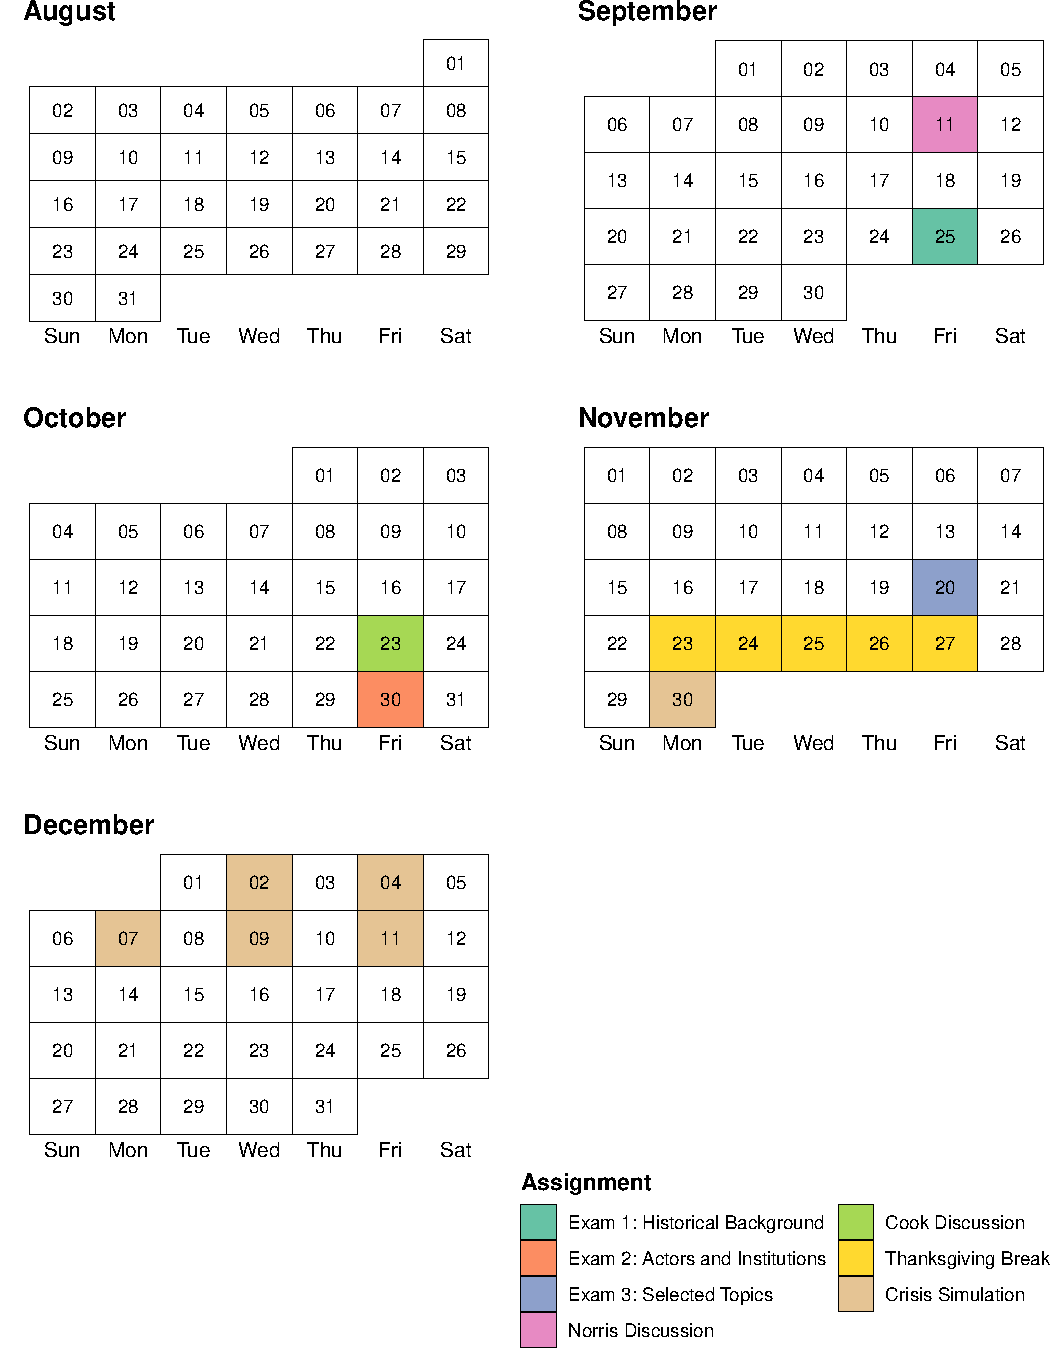
\includegraphics[keepaspectratio]{syllabus-f2026_files/figure-pdf/course-calendar-1.pdf}}
\end{center}

\clearpage

\subsection{Week 01, 08/24 - 08/28: Course Introduction and Historical
Background}\label{week-01-0824---0828-course-introduction-and-historical-background}

\subsubsection{Readings and Assignments}\label{readings-and-assignments}

\begin{itemize}
\tightlist
\item
  \href{https://education.cfr.org/learn/video/why-does-us-foreign-policy-matter}{Why
  does foreign policy matter?}
\item
  \href{https://education.cfr.org/learn/learning-journey/tools-foreign-policy/what-tools-do-foreign-policy-makers-have-at-their-disposal}{What
  tools do foreign policymakers have at their disposal?}
\item
  \href{https://www.archives.gov/founding-docs/declaration-transcript}{Declaration
  of Independence}
\item
  \href{https://www.presidency.ucsb.edu/documents/farewell-address}{Washington's
  Farewell Address}
\item
  \href{https://teachingamericanhistory.org/document/speech-on-independence-day/}{An
  Address\ldots Celebrating the Declaration of Independence}
\item
  \href{https://teachingamericanhistory.org/document/brutus-x/}{Anti-Federalist
  Papers: Brutus X}
\end{itemize}

\subsection{Week 02, 08/31 - 09/04: Historical background
(cont.)}\label{week-02-0831---0904-historical-background-cont.}

\subsubsection{Readings and
Assignments:}\label{readings-and-assignments-1}

\begin{itemize}
\tightlist
\item
  \href{https://www.usmcu.edu/Portals/218/Turner\%20Thesis\%2C\%20Frederick\%20Jackson\%20Turner.pdf}{The
  Significance of the Frontier in American History}
\item
  \href{https://www.archives.gov/milestone-documents/president-woodrow-wilsons-14-points}{Wilson's
  14 Points}
\end{itemize}

\begin{tcolorbox}[enhanced jigsaw, arc=.35mm, bottomrule=.15mm, bottomtitle=1mm, breakable, colback=white, colbacktitle=quarto-callout-important-color!10!white, colframe=quarto-callout-important-color-frame, coltitle=black, left=2mm, leftrule=.75mm, opacityback=0, opacitybacktitle=0.6, rightrule=.15mm, title=\textcolor{quarto-callout-important-color}{\faExclamation}\hspace{0.5em}{\textbf{Friday 09/04: Discussion Day}}, titlerule=0mm, toprule=.15mm, toptitle=1mm]

Readings from Historical Background lectures:

\begin{itemize}
\tightlist
\item
  \href{https://www.archives.gov/founding-docs/declaration-transcript}{Declaration
  of Independence}
\item
  \href{https://www.presidency.ucsb.edu/documents/farewell-address}{Washington's
  Farewell Address}
\item
  \href{https://teachingamericanhistory.org/document/speech-on-independence-day/}{An
  Address\ldots Celebrating the Declaration of Independence}
\item
  \href{https://teachingamericanhistory.org/document/brutus-x/}{Anti-Federalist
  Papers: Brutus X}
\item
  \href{https://www.usmcu.edu/Portals/218/Turner\%20Thesis\%2C\%20Frederick\%20Jackson\%20Turner.pdf}{The
  Significance of the Frontier in American History}
\item
  \href{https://www.archives.gov/milestone-documents/president-woodrow-wilsons-14-points}{Wilson's
  14 Points}
\end{itemize}

\end{tcolorbox}

\subsection{Week 03, 09/07 - 09/11: The Cold War and US
Hegemony}\label{week-03-0907---0911-the-cold-war-and-us-hegemony}

\subsubsection{Readings and
Assignments:}\label{readings-and-assignments-2}

\begin{itemize}
\tightlist
\item
  Read Norris (2021)
\end{itemize}

\subsubsection{Recommended Readings}\label{recommended-readings}

\begin{itemize}
\tightlist
\item
  United States National Security Council (1950)
\item
  Sources, Conduct, and Kennan (1947)
\item
  \href{https://www.archives.gov/milestone-documents/truman-doctrine}{The
  Truman Doctrine}
\end{itemize}

\subsection{Week 04, 09/14 - 09/18: The Cold War and Domestic
Politics}\label{week-04-0914---0918-the-cold-war-and-domestic-politics}

\subsubsection{Readings and
Assignments:}\label{readings-and-assignments-3}

\begin{itemize}
\tightlist
\item
  Dudziak (2004)
\item
  Fordham (2007)
\end{itemize}

\begin{tcolorbox}[enhanced jigsaw, arc=.35mm, bottomrule=.15mm, bottomtitle=1mm, breakable, colback=white, colbacktitle=quarto-callout-important-color!10!white, colframe=quarto-callout-important-color-frame, coltitle=black, left=2mm, leftrule=.75mm, opacityback=0, opacitybacktitle=0.6, rightrule=.15mm, title=\textcolor{quarto-callout-important-color}{\faExclamation}\hspace{0.5em}{Friday 09/18: Discussion Day}, titlerule=0mm, toprule=.15mm, toptitle=1mm]

\begin{itemize}
\tightlist
\item
  Norris (2021)
\end{itemize}

\end{tcolorbox}

\begin{tcolorbox}[enhanced jigsaw, arc=.35mm, bottomrule=.15mm, bottomtitle=1mm, breakable, colback=white, colbacktitle=quarto-callout-important-color!10!white, colframe=quarto-callout-important-color-frame, coltitle=black, left=2mm, leftrule=.75mm, opacityback=0, opacitybacktitle=0.6, rightrule=.15mm, title=\textcolor{quarto-callout-important-color}{\faExclamation}\hspace{0.5em}{\textbf{Friday 09/18: Discussion Day}}, titlerule=0mm, toprule=.15mm, toptitle=1mm]

Readings from Cold War lectures:

\begin{itemize}
\tightlist
\item
  \href{https://www.archives.gov/milestone-documents/truman-doctrine}{The
  Truman Doctrine}
\item
  Dudziak (2004)
\item
  Fordham (2007)
\end{itemize}

\end{tcolorbox}

\subsection{Week 05, 09/21 - 09/25: The Presidency and
Congress}\label{week-05-0921---0925-the-presidency-and-congress}

\subsubsection{Readings and
Assignments:}\label{readings-and-assignments-4}

\begin{itemize}
\tightlist
\item
  Lupton (2017)
\item
  Weissman (2017)
\end{itemize}

\begin{tcolorbox}[enhanced jigsaw, arc=.35mm, bottomrule=.15mm, bottomtitle=1mm, breakable, colback=white, colbacktitle=quarto-callout-important-color!10!white, colframe=quarto-callout-important-color-frame, coltitle=black, left=2mm, leftrule=.75mm, opacityback=0, opacitybacktitle=0.6, rightrule=.15mm, title=\textcolor{quarto-callout-important-color}{\faExclamation}\hspace{0.5em}{Friday 09/25: Exam 1: Historical Background}, titlerule=0mm, toprule=.15mm, toptitle=1mm]

This exam will cover the historical background content from Weeks 1--4.

\end{tcolorbox}

\subsection{Week 06, 09/28 - 10/02: The Policymaking
Process}\label{week-06-0928---1002-the-policymaking-process}

\subsubsection{Readings and
Assignments:}\label{readings-and-assignments-5}

\begin{itemize}
\tightlist
\item
  Miller (2016)
\end{itemize}

\subsection{Week 07, 10/05 - 10/09: The Bureaucracy / The State
Department}\label{week-07-1005---1009-the-bureaucracy-the-state-department}

\subsubsection{Readings and
Assignments:}\label{readings-and-assignments-6}

\begin{itemize}
\tightlist
\item
  \href{https://assets.cfr.org/images/csr89_final/csr89_final.pdf}{Council
  on Foreign Relations: Revitalizing the State Department}
\item
  \href{https://www.nytimes.com/2026/07/11/us/politics/how-marco-rubio-runs-venezuela.html}{New
  York Times: How Marco Rubio Is Running Venezuela From Afar}
\end{itemize}

\begin{tcolorbox}[enhanced jigsaw, arc=.35mm, bottomrule=.15mm, bottomtitle=1mm, breakable, colback=white, colbacktitle=quarto-callout-important-color!10!white, colframe=quarto-callout-important-color-frame, coltitle=black, left=2mm, leftrule=.75mm, opacityback=0, opacitybacktitle=0.6, rightrule=.15mm, title=\textcolor{quarto-callout-important-color}{\faExclamation}\hspace{0.5em}{Friday 10/09: Discussion Day}, titlerule=0mm, toprule=.15mm, toptitle=1mm]

\begin{itemize}
\tightlist
\item
  \href{https://assets.cfr.org/images/csr89_final/csr89_final.pdf}{Council
  on Foreign Relations: Revitalizing the State Department}
\item
  Miller (2016)
\end{itemize}

\end{tcolorbox}

\subsection{Week 08, 10/12 - 10/16: The Defense Department and the
Military}\label{week-08-1012---1016-the-defense-department-and-the-military}

\subsubsection{Readings and
Assignments:}\label{readings-and-assignments-7}

\begin{itemize}
\tightlist
\item
  \href{https://thewarhorse.org/military-standards-women-in-combat/}{The
  War Horse: Women Have Served in Combat Roles for a Decade. The
  Pentagon is Reopening the Debate}
\item
  \href{https://www.military.com/feature/2026/03/24/recruiting-surge-was-engineered-can-it-last-war-iran.html-0}{The
  Recruiting Surge Was Engineered. Can It Last in a War with Iran?}
\item
  \href{https://www.military.com/daily-news/2026/03/11/could-us-bring-back-draft-who-would-be-called-first-and-who-qualifies.html}{Could
  the US Bring Back the Draft? Who Would Be Called First --- and Who
  Qualifies}
\end{itemize}

\begin{tcolorbox}[enhanced jigsaw, arc=.35mm, bottomrule=.15mm, bottomtitle=1mm, breakable, colback=white, colbacktitle=quarto-callout-important-color!10!white, colframe=quarto-callout-important-color-frame, coltitle=black, left=2mm, leftrule=.75mm, opacityback=0, opacitybacktitle=0.6, rightrule=.15mm, title=\textcolor{quarto-callout-important-color}{\faExclamation}\hspace{0.5em}{Friday 10/16: Discussion Day}, titlerule=0mm, toprule=.15mm, toptitle=1mm]

\begin{itemize}
\tightlist
\item
  \href{https://thewarhorse.org/military-standards-women-in-combat/}{The
  War Horse: Women Have Served in Combat Roles for a Decade. The
  Pentagon is Reopening the Debate}
\item
  \href{https://www.military.com/feature/2026/03/24/recruiting-surge-was-engineered-can-it-last-war-iran.html-0}{The
  Recruiting Surge Was Engineered. Can It Last in a War with Iran?}
\item
  \href{https://www.military.com/daily-news/2026/03/11/could-us-bring-back-draft-who-would-be-called-first-and-who-qualifies.html}{Could
  the US Bring Back the Draft? Who Would Be Called First --- and Who
  Qualifies}
\end{itemize}

\end{tcolorbox}

\subsection{Week 09, 10/19 - 10/23: The Use of Military
Force}\label{week-09-1019---1023-the-use-of-military-force}

\subsubsection{Readings and
Assignments:}\label{readings-and-assignments-8}

\begin{itemize}
\tightlist
\item
  Cook (2024)
\item
  Podcast:
  \href{https://warontherocks.com/reopening-the-strait-of-hormuz-saving-downed-pilots/}{War
  on the Rocks: Reopening the Strait of Hormuz \& Saving Downed Pilots}
\item
  \href{https://bbc.com/news/articles/c0qvnk2ezp7o}{As the US pauses the
  war with Iran, is Trump really running out of weapons?}
\item
  Podcast:
  \href{https://mwi.westpoint.edu/mwi-podcast-bunker-busters-and-b-2s/}{Modern
  War Institute Podcast: Bunker Busters and B-2s}
\end{itemize}

\subsubsection{Additional selected
readings:}\label{additional-selected-readings}

\begin{itemize}
\tightlist
\item
  Watch \href{https://watchdocumentaries.com/restrepo/}{Restrepo}
\item
  Read United States Government (2019)
\end{itemize}

\begin{tcolorbox}[enhanced jigsaw, arc=.35mm, bottomrule=.15mm, bottomtitle=1mm, breakable, colback=white, colbacktitle=quarto-callout-important-color!10!white, colframe=quarto-callout-important-color-frame, coltitle=black, left=2mm, leftrule=.75mm, opacityback=0, opacitybacktitle=0.6, rightrule=.15mm, title=\textcolor{quarto-callout-important-color}{\faExclamation}\hspace{0.5em}{Friday 10/23: Discussion Day}, titlerule=0mm, toprule=.15mm, toptitle=1mm]

\begin{itemize}
\tightlist
\item
  Read Cook (2024)
\item
  \href{https://mwi.westpoint.edu/mwi-podcast-bunker-busters-and-b-2s/}{Modern
  War Institute Podcast: Bunker Busters and B-2s}
\end{itemize}

\end{tcolorbox}

\subsection{Week 10, 10/26 - 10/30: Security
Cooperation}\label{week-10-1026---1030-security-cooperation}

\subsubsection{Readings and
Assignments:}\label{readings-and-assignments-9}

\begin{itemize}
\tightlist
\item
  \href{https://www.cfr.org/article/us-aid-israel-four-charts}{Council
  on Foreign Relations: U.S. Aid to Israel in Four Charts}
\item
  \href{https://www.cfr.org/article/how-much-us-aid-going-ukraine}{Council
  on Foreign Relations: Here's How Much Aid the United States Has Sent
  Ukraine}
\item
  \href{https://www.csis.org/analysis/can-ukraine-fight-without-us-aid-seven-questions-ask}{Center
  for Strategic and International Studies: Can Ukraine Fight Without
  U.S. Aid? Seven Questions to Ask}
\item
  \href{https://www.congress.gov/crs-product/R46337}{Congressional
  Research Service: Transfer of Defense Articles: U.S. Sale and Export
  of U.S.-Made Arms to Foreign Entities}
\item
  \href{https://theconversation.com/why-does-the-us-pay-so-much-for-the-defense-of-its-allies-5-questions-answered-127683}{The
  Conversation: Why does the US pay so much for the defense of its
  allies? 5 questions answered}
\item
  \href{https://theconversation.com/the-us-military-presence-in-europe-has-been-declining-for-30-years-the-current-crisis-in-ukraine-may-reverse-that-trend-175595}{The
  Conversation: The US military presence in Europe has been declining
  for 30 years -- the current crisis in Ukraine may reverse that trend}
\end{itemize}

\begin{tcolorbox}[enhanced jigsaw, arc=.35mm, bottomrule=.15mm, bottomtitle=1mm, breakable, colback=white, colbacktitle=quarto-callout-important-color!10!white, colframe=quarto-callout-important-color-frame, coltitle=black, left=2mm, leftrule=.75mm, opacityback=0, opacitybacktitle=0.6, rightrule=.15mm, title=\textcolor{quarto-callout-important-color}{\faExclamation}\hspace{0.5em}{Friday 10/30: Exam 2: Actors and Institutions}, titlerule=0mm, toprule=.15mm, toptitle=1mm]

This exam will cover material on the actors and institutions material
from weeks 5--9.

\end{tcolorbox}

\subsection{Week 11, 11/02 - 11/06: Trade, Finance, and Monetary
Policy}\label{week-11-1102---1106-trade-finance-and-monetary-policy}

\subsubsection{\texorpdfstring{\textbf{No Class on
Friday}}{No Class on Friday}}\label{no-class-on-friday}

\subsubsection{Readings and
Assignments:}\label{readings-and-assignments-10}

\begin{itemize}
\tightlist
\item
  \href{https://tradetalkspodcast.com/podcast/207-what-happened-on-trumps-tariff-day/}{Trade
  Talks: What happened on Trump's tariff day?}
\item
  \href{https://musgrave.substack.com/p/oh-no-i-betrayed-america}{Paul
  Musgrave: Oh no, I betrayed America}
\end{itemize}

\subsection{Week 12, 11/09 - 11/13: Trade, Finance, and Monetary Policy
(cont.)}\label{week-12-1109---1113-trade-finance-and-monetary-policy-cont.}

\subsubsection{Readings and
Assignments:}\label{readings-and-assignments-11}

\begin{itemize}
\tightlist
\item
  \href{https://www.congress.gov/crs_external_products/IF/PDF/IF11751/IF11751.12.pdf}{CRS:
  Introduction to U.S. Economy: Monetary Policy}
\end{itemize}

\begin{tcolorbox}[enhanced jigsaw, arc=.35mm, bottomrule=.15mm, bottomtitle=1mm, breakable, colback=white, colbacktitle=quarto-callout-important-color!10!white, colframe=quarto-callout-important-color-frame, coltitle=black, left=2mm, leftrule=.75mm, opacityback=0, opacitybacktitle=0.6, rightrule=.15mm, title=\textcolor{quarto-callout-important-color}{\faExclamation}\hspace{0.5em}{Friday 11/13: Discussion Day}, titlerule=0mm, toprule=.15mm, toptitle=1mm]

\begin{itemize}
\tightlist
\item
  \href{https://tradetalkspodcast.com/podcast/207-what-happened-on-trumps-tariff-day/}{Trade
  Talks: What happened on Trump's tariff day?}
\item
  \href{https://musgrave.substack.com/p/oh-no-i-betrayed-america}{Paul
  Musgrave: Oh no, I betrayed America}
\item
  \href{https://www.congress.gov/crs_external_products/IF/PDF/IF11751/IF11751.12.pdf}{CRS:
  Introduction to U.S. Economy: Monetary Policy}
\end{itemize}

\end{tcolorbox}

\subsection{Week 13, 11/16 - 11/20: Human Rights
Issues}\label{week-13-1116---1120-human-rights-issues}

\subsubsection{Readings and
Assignments:}\label{readings-and-assignments-12}

\begin{itemize}
\tightlist
\item
  Power (2001)
\item
  \href{https://www.cfr.org/backgrounder/us-immigration-debate-0}{Council
  on Foreign Relations: The US Immigration Debate}
\item
  \href{https://www.nytimes.com/2025/11/08/world/americas/el-salvador-prison-migrants.html}{`You
  Are All Terrorists': Four Months in a Salvadoran Prison}
\end{itemize}

\begin{tcolorbox}[enhanced jigsaw, arc=.35mm, bottomrule=.15mm, bottomtitle=1mm, breakable, colback=white, colbacktitle=quarto-callout-important-color!10!white, colframe=quarto-callout-important-color-frame, coltitle=black, left=2mm, leftrule=.75mm, opacityback=0, opacitybacktitle=0.6, rightrule=.15mm, title=\textcolor{quarto-callout-important-color}{\faExclamation}\hspace{0.5em}{Friday 11/20: Exam 3: Selected Topics}, titlerule=0mm, toprule=.15mm, toptitle=1mm]

This exam will cover all of the special topics material from weeks 9-13.

\end{tcolorbox}

\subsection{Week 14, 11/23 - 11/27: Thanksgiving Break (No
Class)}\label{week-14-1123---1127-thanksgiving-break-no-class}

\subsubsection{Readings and
Assignments:}\label{readings-and-assignments-13}

\begin{enumerate}
\def\labelenumi{\arabic{enumi}.}
\tightlist
\item
  Get some rest
\item
  Enjoy yourselves
\item
  Eat good food
\item
  Take a good nap
\end{enumerate}

\subsection{Week 15, 11/30 - 12/04: Crisis Simulation Week
1}\label{week-15-1130---1204-crisis-simulation-week-1}

\subsubsection{Monday, November 30}\label{monday-november-30}

\begin{itemize}
\tightlist
\item
  Introduce crisis simulation
\item
  Provide overview of the crisis scenario
\item
  Students present initial positions to the President
\end{itemize}

\subsubsection{Wednesday, December 2}\label{wednesday-december-2}

\begin{itemize}
\tightlist
\item
  Review proposals
\item
  Clarify obstacles, risks, benefits, opportunities, threats, etc.
\item
  Evaluate positions
\end{itemize}

\subsubsection{Friday, December 4}\label{friday-december-4}

\begin{itemize}
\tightlist
\item
  Narrow the options
\item
  Provide time for groups to discuss changes with one another
\end{itemize}

\subsection{Week 16, 12/07 - 12/11: Crisis Simulation Week
2}\label{week-16-1207---1211-crisis-simulation-week-2}

\subsubsection{Monday, December 8, 2025}\label{monday-december-8-2025}

\begin{itemize}
\tightlist
\item
  Introduce crisis simulation
\item
  Provide overview of the crisis scenario
\item
  Students present initial positions to the President
\end{itemize}

\subsubsection{Wednesday, December 10,
2025}\label{wednesday-december-10-2025}

\begin{itemize}
\tightlist
\item
  Review proposals
\item
  Clarify obstacles, risks, benefits, opportunities, threats, etc.
\item
  Evaluate positions
\end{itemize}

\subsubsection{Friday, December 12, 2025}\label{friday-december-12-2025}

\begin{itemize}
\tightlist
\item
  Reflection Day
\item
  Complete reflection memo
\item
  What worked?
\item
  What didn't work?
\item
  What about the process surprised you?
\end{itemize}

\protect\phantomsection\label{refs}
\begin{CSLReferences}{1}{1}
\bibitem[\citeproctext]{ref-Cook2024}
Cook, Steven A. 2024. \emph{The {End} of {Ambition}: {America}'s {Past},
{Present}, and {Future} in the {Middle East}}. Oxford, New York: Oxford
University Press.

\bibitem[\citeproctext]{ref-Dudziak2004}
Dudziak, Mary L. 2004. {``Brown as a {Cold War Case}.''} \emph{The
Journal of American History} 91(1): 32--42.
\url{https://www.jstor.org/stable/3659611} (August 18, 2021).

\bibitem[\citeproctext]{ref-Fordham2007}
Fordham, Benjamin O. 2007. {``The Evolution of Republican and Democratic
Positions on Cold War Military Spending.''} \emph{Social Science
History} 31(4): 603--36.

\bibitem[\citeproctext]{ref-Lupton2017}
Lupton, Danielle L. 2017.
{``\href{https://doi.org/10.1177/1065912917691359}{Out of the {Service},
{Into} the {House}: {Military Experience} and {Congressional War
Oversight}}.''} \emph{Political Research Quarterly} 70(2): 327--39.

\bibitem[\citeproctext]{ref-Miller2016}
Miller, Paul D. 2016.
{``\href{https://doi.org/10.1080/01402390.2016.1145588}{Graveyard of
{Analogies}: {The Use} and {Abuse} of {History} for the {War} in
{Afghanistan}}.''} \emph{Journal of Strategic Studies} 39(3): 446--76.

\bibitem[\citeproctext]{ref-Norris2021}
Norris, John. 2021. \emph{The {Enduring Struggle}: {The History} of the
{U}.{S}. {Agency} for {International Development} and {America}'s
{Uneasy Transformation} of the {World}}. Lanham, Maryland Boulder, Colo.
New York,NY London: Rowman \& Littlefield Publishers.

\bibitem[\citeproctext]{ref-Power2001}
Power, Samantha. 2001. {``Bystanders to Genocide: {Why} the United
States Let the Rwandan Tragedy Happen.''} \emph{The Atlantic Monthly}:
84--108.

\bibitem[\citeproctext]{ref-Kennan1947}
Sources, The, Soviet Conduct, and George F Kennan. 1947. {``The Sources
of Soviet Conduct.''} \emph{Foreign Affairs} 25(4): 566--82.

\bibitem[\citeproctext]{ref-sigar2019}
United States Government. 2019. \emph{Divided {Responsibility}:
{Lessons} from {U}.{S}. {Security Sector Assistance Efforts} in
{Afghanistan}}. Special Inspector General for Afghanistan
Reconstruction.

\bibitem[\citeproctext]{ref-NSC68}
United States National Security Council. 1950. \emph{{NSC-68}}. United
States Government.

\bibitem[\citeproctext]{ref-Weissman2017}
Weissman, Stephen R. 2017. {``Congress and {War}: {How} the {House} and
the {Senate Can Reclaim Their Role}.''} \emph{Foreign Affairs} 96(1):
132--45. \url{https://www.jstor.org/stable/44823238} (August 18, 2025).

\end{CSLReferences}




\end{document}
